\documentclass{ba-kecs}
\usepackage{graphicx,, url}
\usepackage[numbers]{natbib}
\usepackage{amssymb,amsmath}

\title{Turtlebot SLAM }

\author{Maurice Hermans, Lukas Kang, Michael Norget, Thomas Nowicki, Oliver Trinnes}

\begin{document}

\maketitle

\begin{abstract}
This article accompanies the research project "TurtleBot SLAM" from the Master "Artificial Intelligence" of Maastricht University.
\end{abstract}

\section{Introduction}
Nowadays mobile robots are able to assist humans in a diverse set of problems. Transportation, search, rescue and automated vacuum cleaning are examples from different fields. Typically, mobile robots can move through an environment using legs or wheels. In addition they are able to gather information about their environment using sensors. Some even have devices similar to the human arm or hand which allows them to interact with the environment. The vaccuum cleaning robot presented in Figure \ref{fig:vacuum_cleaner} is an example of a robot which has whells to move around. Furthermore it is equipped with a set of sensors. These sensors provide data about the location of obstacles as well as, for example, gaps in the floor the robot is moving on. To efficiently perform this task robots needs a map of its environment. For some tasks map data is available for the robot from the beginning. Provided a map the robot can locate itself using the incoming sensor data. For tasks in unknown environments, however, the robot must rely on internal sensors and make its own map of the environment.

The acquisition of these maps has been a major research focus in the robotics community \cite{Grisetti} [\textbf{MORE SOURCES}]. Building or learning these maps under position uncertainty provided only sensor measurements is often referred to as the Simultaneous Localization And Mapping (SLAM) problem. A large variety of solutions is available to the SLAM problem, these approaches can be classified as either filtering or smoothing [\textbf{SOURCE}].

Filtering approaches model the problem as a so called ``on-line" state estimation problem. The state of such a system consists of the current robot position and the map. New measurements augment and refine the estimate as they become available. Due to their incremental nature these filtering approaches are commonly referred to as on-line SLAM methods. The other type of approach estimates the full trajectory from the full set of measurements. These approaches address the so called full SLAM problem and they typically rely on least-square error minimization techniques [\textbf{SOURCE}].

An intuitive way to formulate the SLAM problem is to consider it as a pose graph optimization problem. The nodes of the graph represent robot poses or landmarks. The edges encode sensor measurements that constraint the connected poses. Once such a graph is constructed the graph-based SLAM method tries to find a configuration of the nodes that is maximally consistent with the contraints contained in the edges. (\textbf{abstract graph picture here})

The rest of this paper is structured as follows. Section \ref{sec:sota} provides the reader with the necessary background information on the topic. Section \ref{sec:impl} is about the implementation details of the methods used. Section \ref{sec:exp} explains the experiments ran to validate and benchmark the implemented methods and also evaluate the obtained results. Section \ref{sec:disc} discusses the acquired results of the experiments and proposes further research based on those. And the last section wraps up the paper with the conclusions of this research.

\begin{figure}[htp]
	\centering
		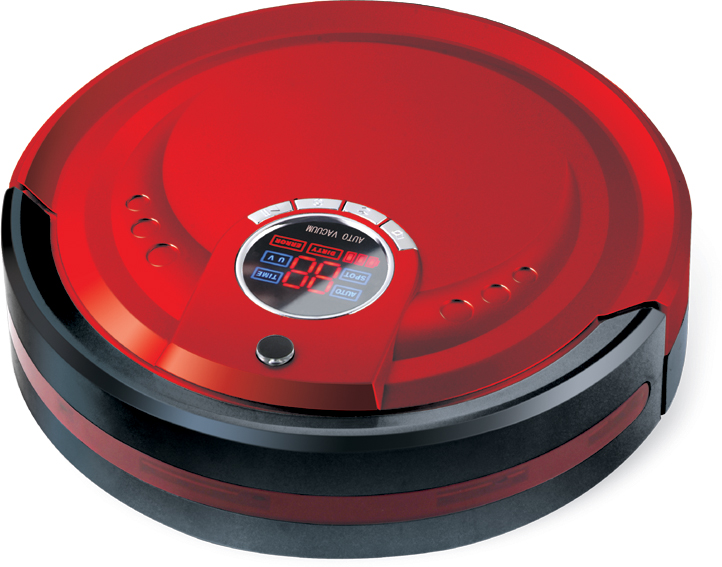
\includegraphics[width=0.50\textwidth]{figures/vacuum_cleaner.jpg}
	\caption{Automated vacuum cleaner}
	\label{fig:vacuum_cleaner}
\end{figure}

\subsection{Problem Statement}
The focus of this paper is SLAM, more specifically GraphSLAM and how it is used to construct a map of an unknown environment. GraphSLAM returns as a result the optimized graph representing the path the robot has explored. Because the goal of the robot in this paper is to map the entire area where it has been placed. There is also the need for an exploration strategy to map the still unseen areas of the space where the robot is located. The results returned by the GraphSLAM algorithm are turned into an occupancy grid map and then used for the autonomous exploration. The algorithm is tested in a robot simulator called STAGE which simulates a provided map.

\section{State of the art}
\label{sec:sota}
\subsection{ROS}
ROS (Robot Operating System) \cite{Quigley}, is the framework used in this paper to program the robots and it provides an environment to run simulations for the implemented algorithm. As described by Quigley et al. \cite{Quigley}, writing software for robots is difficult since there are so many possible hardware setups which makes code reuse nontrivial. Adding to this problem of hardware setups is the amount of code needed as it must contain a deep stack starting from driver-level software going up through perception, abstract reasoning and beyond. Since the required expertise is well beyond the capabilities of a single researcher, robotics software architectures must also support large scale software integration efforts.

To deal with the above mentioned problems many robotics researchers have created a wide variety of frameworks to deal with this complexity and facilitate them with the needs for their own research. This resulted in the many robotic software systems currently used by academia and industry \cite{Kramer}. Each of these frameworks was designed for a specific purpose, perhaps the available frameworks did not meet the requirements this researcher had or the emphasis was on the wrong aspects according to the researcher.

The ROS framework used in this paper is also the product of trade-offs and prioritizations. The emphasis of this framework is on large-scale integrative robotics research, making it useful in a wide variety of situations.

\subsection{TurtleBot}
The robots on which the algorithm from this paper will be tested are called TurtleBots, see figure \ref{fig:turtlebot}, the simulator will also mimic these robots. The TurtleBot is a low-cost, customizable, personal robot kit with open-source software. As a base iRobot Create is used (A) which holds a battery pack and 150 degrees/second Single Axis Gyro. The model shown in figure  \ref{fig:turtlebot} uses a Microsoft Kinect as sensor (B), the one used in this paper uses a laser range sensor, and a laptop (C) to run all the processes. The robot can also be customized using the mounting hardware (D). The robot runs on an open-source SDK based on ROS which integrates all the software needed to get the TurtleBot running and already includes some advanced capabilities like mapping and navigation.

\begin{figure}[h]
	\centering
		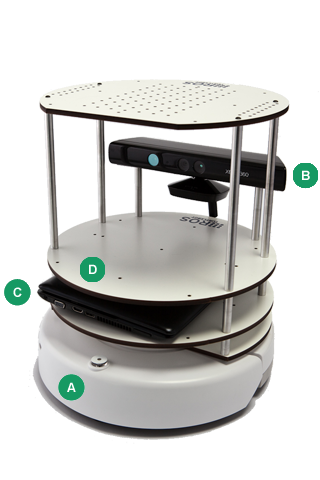
\includegraphics[width=0.50\textwidth]{figures/turtlebot.png}
	\caption{A TurtleBot}
	\label{fig:turtlebot}
\end{figure}

\subsubsection{TurtleBot simulator}
To help with development a simulator is used to simulate the TurtleBots, the one used in this paper is called Stage. In stage it is possible to load layouts of rooms, called worlds, to simulate the robot being placed there. Once a world is loaded into stage one can drive around using manual or autonomous navigation. In stage it is possible to visualize the data the robot uses, for example the laser scans it is measuring or the path it has traveled. Then there is another tool to visualize the output of the algorithm the robot is performing, the 3D visualization tool rviz. This tool helps to evaluate and validate the output returned when performing the GraphSLAM algorithm.

\subsection{Exploration}
Many robots can navigate using maps provided to them, usually the mapping is done by humans before the robot is send to perform its task, this however limits the robot in its ability to navigate in unknown environments. The robots discussed in this paper however do not know anything of their environment at the start and need to build their own map. Thats why robots should be able to explore their environment, which we will define as the act of moving through an unknown environment while building a map that will be used for subsequent navigation. A good exploration strategy is one that generates a (nearly) complete map in the shortest amount of time.

Since the robot does not know anything about its environment the central idea is that it should move to where it would gain as much information as possible. This target should be extracted from the information the robot has obtained so far. Initially the robot knowns nothing except what is measures with its sensors. The map the robot creates should be as complete as possible and build as quickly as possible.

To achieve this the robot makes use of the idea of frontier-based exploration, first introduced by Yamauchi \cite{Yamauchi}. Frontiers are regions on the boundaries between open explored and unexplored space. When a robot moves to a frontier it will take measurements of unexplored space and add this new information to its map. As a result the explored region on the map expands and new frontiers are added to the map. By constantly moving to frontiers the robot can keep expanding its knowledge about the environment. Note that when the robot detects an obstacle there will be no frontiers behind them since it is no region separating open explored from unexplored space.

The performance of the exploration is then not only depending on the strategy the robot uses to select frontiers to explore but also on how to incorporate the new information into the map. This is a challenge since all the new information obtained is effected by noise, not only on the sensor measurements but also on the odometry data used to incorporate newly obtained information.

\subsection{SLAM}
To navigate through an unknown environment a robot needs to be able to build a map of the environment and simultaneously be able to localize itself within this map. This is called Simultaneous Localization And Mapping (SLAM). It basically means that the robot should be able to learn the map under pose uncertainty.

A large variety of solutions is available to the SLAM problem. These approaches can be classified into two categories, namely filtering and smoothing. 

The filtering approaches make a state estimation where the state of the system are stored in the current position and the map. New measurements are incorporated as they become available. In this category fall popular techniques like Kalman filters, particle filters, or information filters.

Conversely, the smoothing approaches keep using all measurements to estimate the entire trajectory the robot has traveled.

\subsubsection{GraphSLAM}
An intuitive way to address the SLAM problem is to pose it as a graph optimization problem. A graph will be constructed where the nodes represent robot poses or landmarks and where edges correspond to measurements that constraint the connecting nodes. Note that constraints can be contradictory because of the noise on the measurements. Once a graph is constructed the algorithm will try to find a configuration of the nodes that is maximally consistent with the measurements.

\section{Implementation}
\label{sec:impl}

The implementation used for this paper is written on a Linux operating system. Programming has been done using ROS and the object oriented programming language C++. The installation process for ROS, as done in this paper, can be reviewed on Maastricht's swarmlab homepage \cite{swarmlab}.
 For the coding part there exist two main packages, one of which includes the exploration and the other one the mapping part of the SLAM problem. To enable the robot with exploration capabilities, the ROS internal navigation stack for the TurtleBot has been used, making movement possible by sending a designated goal to the robot.

\subsection{Wavefront frontier detection}

As a part of the assignment the robot has to drive autonomously through an unknown map. This feature is implemented using Wavefront frontier detection (WFD).

WFD is using frontiers for its exploration purposes. Creation of frontiers requires the robot to know about the current environment in form of a map. In this example an Occupancy grid is used \ref{sec:mapping}. The general algorithm is then used to acquire four different data structures that store map and frontier information. These four data structures are :

1. Map-Open-List
\newline
2. Map-Close-List
\newline
3. Frontier-Open-List
\newline
4. Frontier-Close-List 
\newline
 
To understand the need of these four structures it is necessary to know that WFD is using a breadth first search (BFS), starting at the current robot position that has to be passed into the function. WFD also requires a current map representation, in this program acquired by the mapping package.
 Upon launching the algorithm it first searches for unoccupied space around the current robot location, which is then saved into the Map-Open-List. 
 Frontiers are found by making use of the occupancy grid's structure. A criterion for a point to be a frontier is that it has to have unknown space and known unoccupied space around it. If a frontier point is found a new BFS is performed, to extract all adjacent frontier points and connect them to one consistent frontier into the Frontier-Open-List.
 The benefit of using WFD is that by maintaining these lists, rescans only need to incorporate points that have not been scanned yet, as the algorithm saves once detected open space and frontiers into its adjacent close lists. For upfollowing scans these points are then no longer considered and by that the algorithm is optimized.
 
 Detecting frontiers and navigating towards them is not possible due to ROS's navigation stack. Instead of sending the robot the goal to a frontier point, an algorithm has to be performed to find a point next to the frontier cell with as much free space around it as possible. 
\subsection{GraphSLAM}
Two different approaches of graph-based SLAM are implemented for this project. They differ in complexity and thereby applicability to the problem. Both algorithms create an occupancy grid map. 

First, an algorithm as suggested by \citep{Grisetti} is implemented. Here the graph consists of nodes representing positions along the robot trajectory. Odometry and sensor measurements are incorporated into the constraints contained in the edges. Again, an edge connects two adjacent poses of the robot. This graph-based SLAM approach optimizes the pose graph according to the constraints. This ``optimized" trajectory then determines the positions of obstacles on the map by refining the laser scan data according to the poses they were obtained at. Each edge thus is labelled with the spatial difference between two poses \(x_i\) and \(x_j\). Let this error be denoted by \(e_{ij}(x_i, x_j)\). This graph-based SLAM approach calculates the most likely path as follows:
First it calculates the Jacobians \(A\) and \(B\) of every two estimated positions connected by an edge.
\begin{equation}
\label{eq:jacobi_a}
	A_{ij} = \frac{\partial e_{ij}(x)}{\partial x_i}\uplus
\end{equation}
\begin{equation}
\label{eq:jacobi_b}
	B_{ij} = \frac{\partial e_{ij}(x)}{\partial x_j}
\end{equation}
Note that in Equations \ref{eq:jacobi_a} and \ref{eq:jacobi_b} the x represents the current guess of the concerning robot position. These Jacobians are then added to an information matrix \(H\) (see Equation \ref{eq:H}).
\begin{equation}
\label{eq:H}
\begin{aligned}
	H_{[ii]} += A^{T}_{ij} \Omega_{ij} A_{ij} \\
	H_{[ij]} += A^{T}_{ij} \Omega_{ij} B_{ij} \\
	H_{[ji]} += B^{T}_{ij} \Omega_{ij} A_{ij} \\
	H_{[jj]} += B^{T}_{ij} \Omega_{ij} B_{ij} \\
\end{aligned}
\end{equation}
Furthermore a coefficient vector \(b\) is always updated as shown in Equation \ref{eq:b}. This vector in combination with the \(H\) matrix form a set of linear constraints.
\begin{equation}
\label{eq:b}
\begin{aligned}
	b_{[i]} += A^{T}_{ij} \Omega_{ij} e_{ij} \\
	b_{[j]} += B^{T}_{ij} \Omega_{ij} e_{ij} 
\end{aligned}
\end{equation}
Optimizing the vector \(x = (x_1, ..., x_n)^T \) according to the constraints specified in \(H\) and \(b\) is the core of this approach. This step is performed using sparse Cholesky factorization. 
A new node is added to the graph once the robot moved 0.5 meters. The algorithm optimizes the trajectory like explained when a new node is added. In one special case the algorithm adds and edge connecting to non-adjacent nodes to the graph. This happens when the distance between the two connected robot positions is smaller than a margin. In fact, this special case enables the algorithm to create loops in the graph and more accurately estimate the robots trajectory and the map. This procedure is referred to as ``loop closing". 
\\
\\
The second implementation is based on \cite{Thrun}. It creates nodes for each odometry measurement of the robot as well as for each feature in the map spotted by the laser sensor. Each occupancy grid cell containing an obstacle is considered a map feature. Edges are labelled with spatial constraints of the two nodes they are connecting. The output of this implementation is a vector containing the positions of the land marks as well as the trajectory of the robot. Here the constraints labelling the edges ar created using Jacobians similar to the previous approach. The major difference lies in the node creation. Here nodes are added for landmarks while the previous implementation considered the robots' trajectory only. Since no obstacle in the final occupancy grid must be missed all obstacle points are treated as landmarks for this implementation. 
\subsubsection{Scan matching}

The scan matcher, used by this program, is necessary to acquire an optimized movement vector between two robot positions, which is needed by the GraphSLAM algorithm. The programming of the scan matcher used requires two steps. For the first step the two scans are matched together by making use of raw odometry data, retrieved by the robot's motion sensor. The improvement done by the scan matcher is then to run an iteration of the iterative closest point algorithm (ICP), to incorporate its perception with the movement. 

The general procedure of the algorithm is to first find corresponding neighbors. These are found by using the nearest neighbor search. Points in this implementation can have multiple correspondences to neighbors. To avoid incorporating outlying points, a fixed distance has been set. Outliers would otherwise impact further calculations negatively.
The next step in the process is to calculate center points for both clouds, which are needed to normalize both clouds in respect ot each other. After performing the calculation the center points for each cloud are subtracted from every point belonging to that cloud. The calculated points are then added to two seperate matrizes, both representing one point cloud. The first cloud's matrix is then multiplied by the transposition of the second cloud matrix, so that a new Matrix is created for which we calculate the SVD values to retrieve a rotational matrix, responsible for rotating the second point cloud to the first one.
\subsection{Mapping}\label{sec:mapping}

For Mapping purposes an Occupancy grid is created on which information about obstacles, free/- and unknown space is saved. Using ROS's visualization program, RVIZ, the map can be visualized entirely.

The occupancy grid is a structure that can be represented by a single dimensional array. Its size is responsible for the size of the grid and is often problem specific, especially for the purpose of Slam. Making the grid too large can lead to performance problems and by that the grid's size gets to be a tunable parameter that has to be chosen carefully for each problem, although making the grid large prevents the robot from going ``out of space''.
 This program converts the array into a two dimensional representation, so that navigating to either side gets more intuitive. Each value of the array is an integer and represents the current status of the cell. The value ranges for ROS's occupancy grid lie between $-1$ and $100$ \cite{occupancy}. Each value has its own meaning :

\begin{description}
\item{$-1$} : unknown space, not yet covered by robot's perception sensors
\item{$ 0$} : known free space, robot can drive on it safely
\item{$1-100$} : probability of being an obstacle, $1$ being a low probability and $100$ being a definite obstacle
\end{description}

\begin{figure}[htbp]
	\centering
		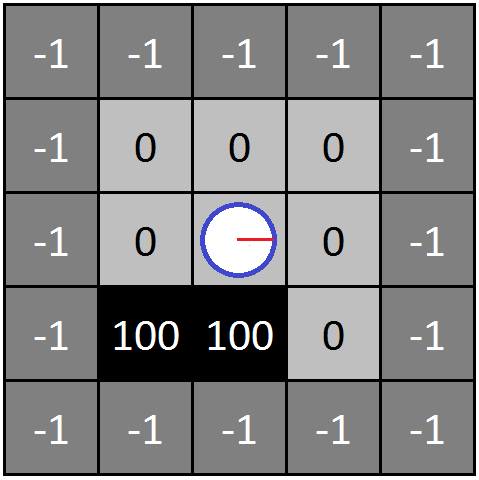
\includegraphics[width=0.50\textwidth,height = 44mm]{figures/Occup.png}
	\caption{Occupancy Grid visualized}
	\label{fig:Occupancy}
\end{figure}
Fig.\ref{fig:Occupancy} shows these three occurrences visualized, with a robot in the middle performing a sample scan of its environment.
The occupancy grid is using laser scan data for this implementation. Each laser scan has information about whether an obstacle has been detected, or whether the maximum range of the scan has been reached. The scan is then transformed into a point cloud to extract its coordinate information and by that, obstacles can be found.

Free space is being incorporated into the map by filling the occupancy grid between a detected obstacle, or detected maximum range point and the current robot position with $0$ values. This is achieved with the help of a linear function. If a point is not the scanner's maximum range away, the point is saved as an obstacle with value $100$.

As time progresses and the robot explores more of its environment the map is constantly updated. This is programmed by saving laser scans for every pose of the robot, which, when traveling for a distance of $0.5$ meters is added and by that the occupancy grid is updated. Upon a loop closure the occupancy grid is optimized with its information about obstacles and free spaces.

\section{Experiments and Results}
\label{sec:exp}
This section demonstrates the results of the Turtlebot SLAM implementation as described in section \ref{sec:impl}. Several outputs of the visualization tool RViz are presented and discussed. Comparisons are drawn between different variations of the implementation and the performance of the program is evaluated.

\subsection{Visualization}
When running the program via the launch file, RViz and Stage are automatically started. Stage shows the robot in its actual position on an accurate test map (see figure \ref{fig:stage_and_rviz} left). RViz shows the current belief of the robot about its environment, position and trajectory (see figure \ref{fig:stage_and_rviz} right). The nodes of the pose graph are visualized by green points and red arrows indicating the past orientation of the robot in this position. The constraints between the nodes are visualized by lines connecting the poses. The yellow points represent the frontier points that have been detected, the orange point being the one the robot is currently navigating to. The acquired information about the environment is displayed as an occupancy grid containing obstacles (black), free space (light gray) and unknown space (dark gray).

\begin{figure}[htbp]
	\centering
		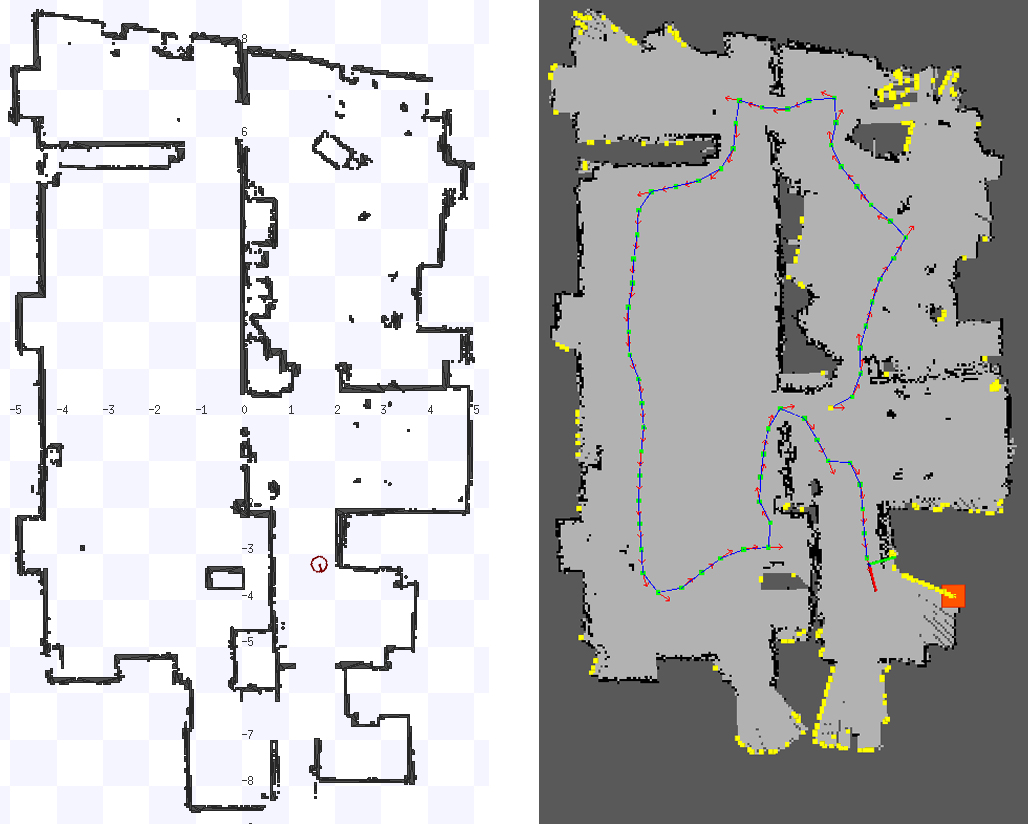
\includegraphics[width=0.50\textwidth]{figures/Stage_and_rviz.jpg}
	\caption{Robot and environment visualization with Stage (left) and RViz (right)}
	\label{fig:stage_and_rviz}
\end{figure}

\subsection{Loop closing effect}

\begin{figure}[htbp]
	\centering
		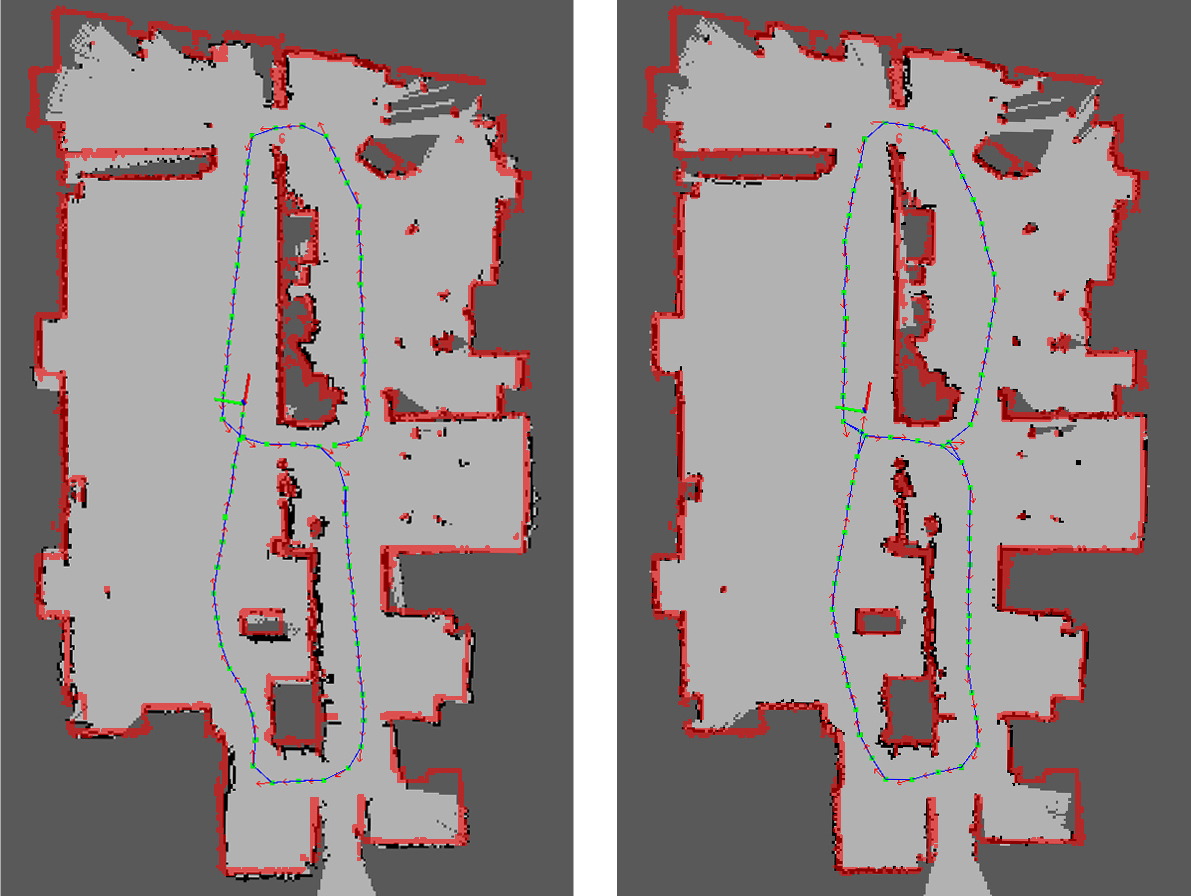
\includegraphics[width=0.50\textwidth]{figures/Loop_closing_compared.jpg}
	\caption{Observed environment without (left) and with (right) loop closing of the pose graph}
	\label{fig:loop_closing_comparison}
\end{figure}

\subsection{Navigation evaluation}

\begin{figure}[htbp]
	\centering
		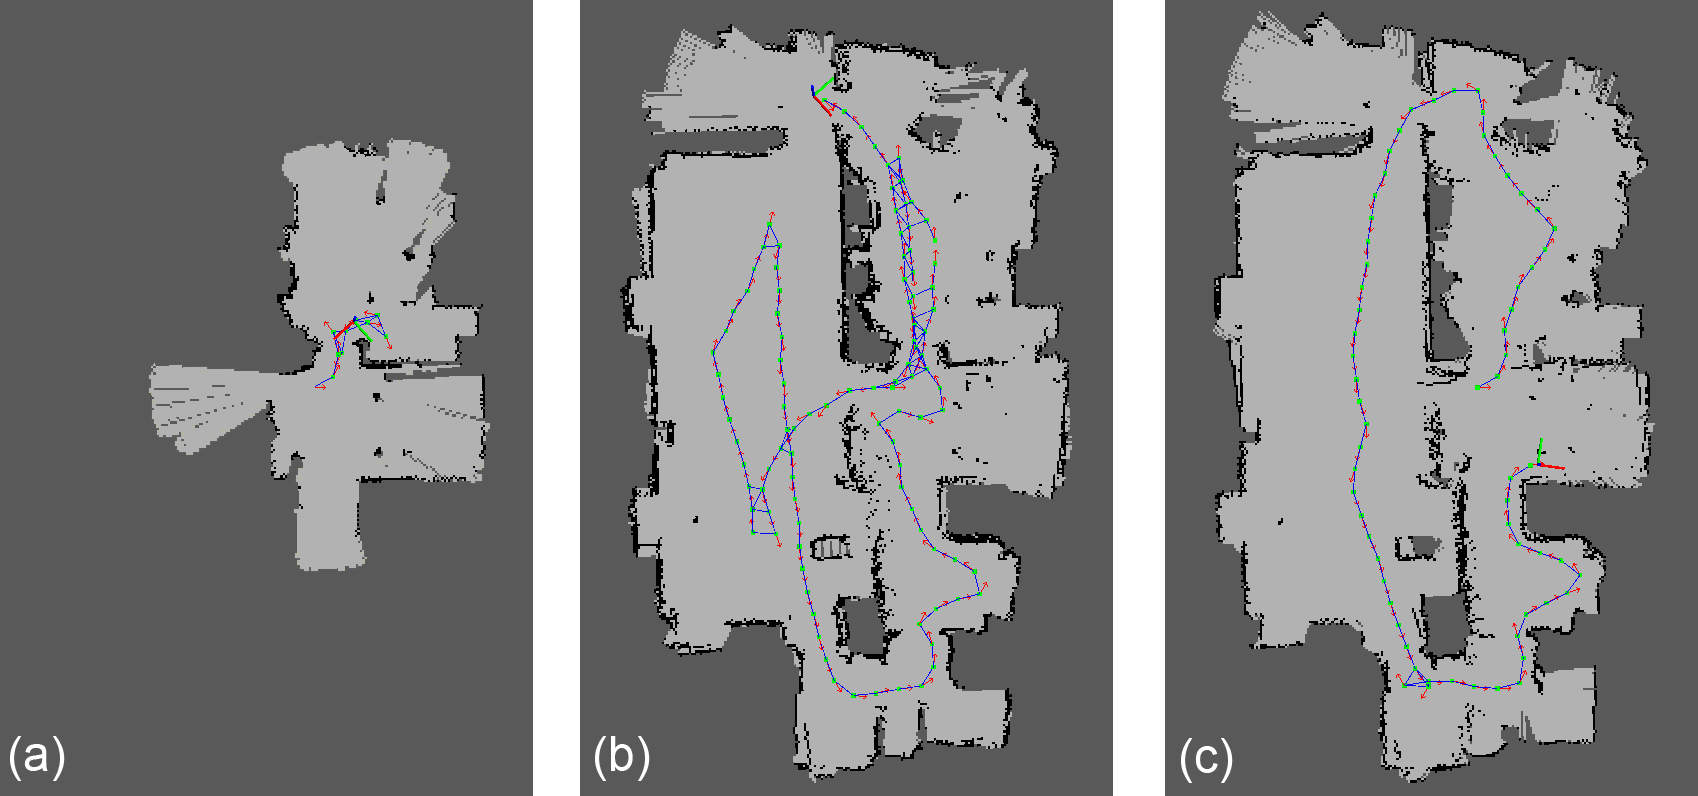
\includegraphics[width=0.50\textwidth]{figures/Navigation_comparison.jpg}
	\caption{Resulting robot trajectory when applying different strategies for selecting the next navigation goal}
	\label{fig:navigation_comparison}
\end{figure}

\subsection{Runtime}

\section{Discussion}
\label{sec:disc}
The Wavefront Frontier detection algorithm \citep{Keidar} succeeds in finding frontiers in a fast and accurate manner.

Implementing the algorithm suggested in \citep{Grisetti} turned out to be well suited for attacking the problem statement of this project. The maps created by this algorithm look accurate. Specifically the margin between the output map and the real map is negligible (FIGURE???). Maps are created in real time and loop closures are added when needed. In fact, the algorithm keeps updating the map with no noticable delay while the robot drives around steering to new goals selected by the WFD algorithm and navigated by ROS' move\_base package.

The second graph-based SLAM implementation \cite{Thrun} clearly is not suited for robots equipped with laser scanners only. Extensive feature extraction methods are required to create occupancy grid maps with the used TurtleBot. Furthermore the algorithm is expected to work best with a robot which is able to detect distinct landmarks as well as a simple environment. A number of unique landmarks can then serve as orientation points to build the map. Additionally the algorithm is able to assess map and trajectory more quickly if there are fewer nodes and constraints in the graph.

\subsubsection{Future research}

\section{Conclusion}
\label{sec:conc}
\bibliography{references}
\nocite{*}
\onecolumn
\appendix

\end{document}
